\documentclass[a4paper,12pt]{article}

%%% Работа с русским языком
\usepackage{cmap}					% поиск в PDF
\usepackage{mathtext} 				% русские буквы в формулах
\usepackage[T2A]{fontenc}			% кодировка
\usepackage[utf8]{inputenc}			% кодировка исходного текста
\usepackage[english,russian]{babel}	% локализация и переносы
\usepackage{xcolor}
\usepackage{hyperref}
 % Цвета для гиперссылок
\definecolor{linkcolor}{HTML}{799B03} % цвет ссылок
\definecolor{urlcolor}{HTML}{799B03} % цвет гиперссылок

\hypersetup{pdfstartview=FitH,  linkcolor=linkcolor,urlcolor=urlcolor, colorlinks=true}

%%% Дополнительная работа с математикой
\usepackage{amsfonts,amssymb,amsthm,mathtools} % AMS
\usepackage{amsmath}
\usepackage{icomma} % "Умная" запятая: $0,2$ --- число, $0, 2$ --- перечисление

%% Номера формул
%\mathtoolsset{showonlyrefs=true} % Показывать номера только у тех формул, на которые есть \eqref{} в тексте.

%% Шрифты
\usepackage{euscript}	 % Шрифт Евклид
\usepackage{mathrsfs} % Красивый матшрифт

%% Свои команды
\DeclareMathOperator{\sgn}{\mathop{sgn}}

%% Перенос знаков в формулах (по Львовскому)
\newcommand*{\hm}[1]{#1\nobreak\discretionary{}
{\hbox{$\mathsurround=0pt #1$}}{}}
% графика
\usepackage{graphicx}
\graphicspath{{pictures/}}
\DeclareGraphicsExtensions{.pdf,.png,.jpg}
\author{Бурмашев Григорий, БПМИ-208}
\title{Матан, дз -- 9}
\date{\today}
\begin{document}
\maketitle
\clearpage
\section*{Номер 1}
\[
f(x) = x \cos x, \; [0, \pi ]
\]
Хотим четность на $[-\pi, \pi]$, тогда дополним нашу функцию для четности:
\[
\tilde{f}(x) = 
\begin{cases}
x \cos x, \; [0, \pi ] \\ 
-x \cos x, \; [-\pi, 0] 
\end{cases}
\]
Тогда получим график вида:
\begin{center}
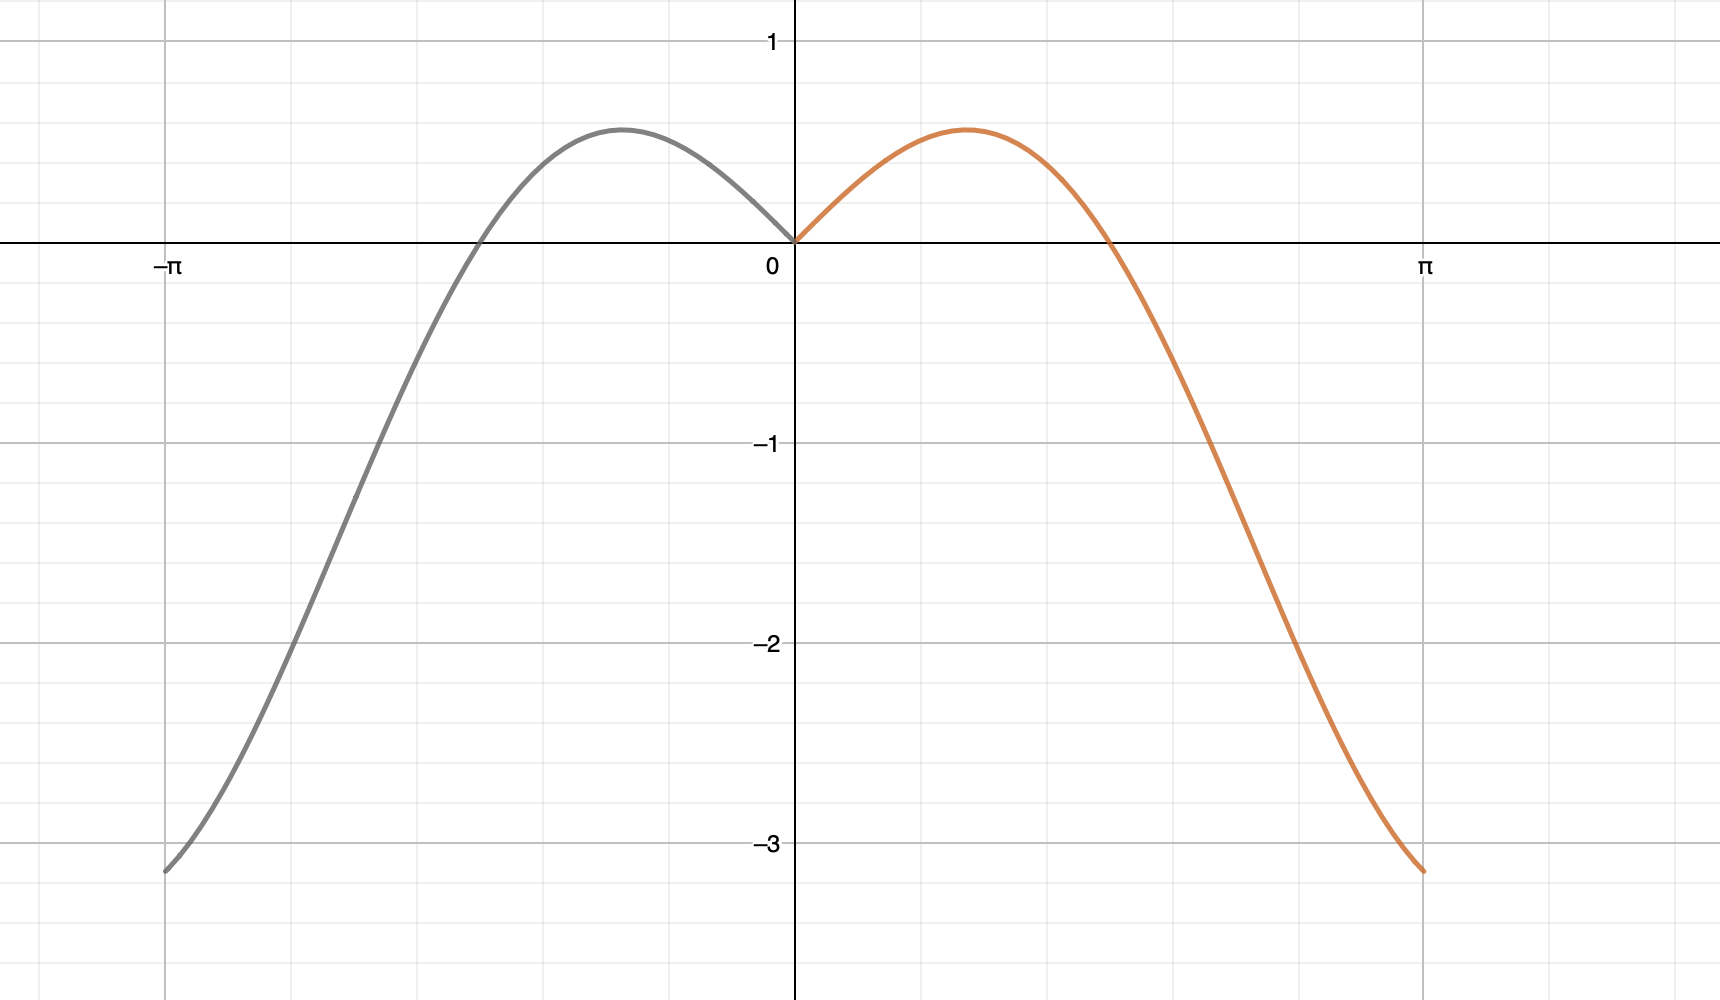
\includegraphics[scale=0.3]{1.png}
\end{center}
$\tilde{f}$ на $[-\pi, \pi]$ -- четная, тогда:
\[
a_0 = \frac{1}{\pi} \int\limits_{-\pi}^{\pi} \tilde{f}(x) dx  = \frac{2}{\pi} \int\limits_{0}^{\pi} \tilde{f}(x) dx =  \frac{2}{\pi} \int\limits_{0}^{\pi} x \cos x dx = \frac{2}{\pi} \left(
x \sin x \Bigg|_0^{\pi} - \int\limits_0^{\pi} \sin x dx
\right) = \frac{2}{\pi} \cdot (-2)  = - \frac{4}{\pi}
\]
\[
a_k = \frac{2}{\pi} \int\limits_{0}^{\pi} \tilde{f}(x) \cos  (kx)  dx  = \frac{2}{\pi} \int\limits_{0}^{\pi} x \cos x\cos  (kx)  dx = \frac{2}{2\pi} \int\limits_{0}^{\pi} x \cdot \left( \cos(kx + x)  + \cos(x - kx) \right) dx  = 
\]
\[
= \frac{1}{\pi} \int\limits_0^{\pi} x \cdot \cos (x + kx) dx + \frac{1}{\pi} \int\limits_0^{\pi} x \cdot \cos (x - kx) dx  = (\times)
\]
Посчитаем эти интегралы отдельно:
\[
\int\limits_0^{\pi} x \cdot \cos (x + kx) dx = \frac{x \sin (x + kx)}{k + 1} \Bigg|_0^{\pi} - \frac{1}{k + 1} \int\limits_0^{\pi} \sin (x + kx) dx  = -\frac{\pi \sin (\pi k)}{k + 1} + \frac{\cos (x + kx)}{(k+1)^2} \Bigg|_0^{\pi} = 
\]
\[
= -\frac{\pi \sin (\pi k)}{k + 1} + \frac{\cos (\pi (k + 1)) -1}{(k+1)^2} = 0 + \frac{(-1)^{k+1} - 1}{(k+1)^2}
\]
\[
 \int\limits_0^{\pi} x \cdot \cos (x - kx) dx  = 0 - \frac{1 + \cos (\pi k)}{(k-1)^2} = - \frac{(-1)^{k} + 1}{(k-1)^2}
\]
Возвращаемся:
\[
(\times) = \frac{1}{\pi} \cdot \left(\frac{(-1)^{k+1} - 1}{(k+1)^2}\right) + \frac{1}{\pi} \cdot \left( - \frac{(-1)^{k} + 1}{(k-1)^2}\right) = \frac{1}{\pi} \cdot \left(\frac{(-1)^{k+1} - 1}{(k+1)^2}  - \frac{(-1)^{k} + 1}{(k-1)^2}
\right)
\]
Видим проблемную точку $k = 1$, где знаменатель уходит в ноль, посмотрим отдельно:
\[
a_1 = \frac{2}{\pi} \int\limits_{0}^{\pi}  x \cos^2 (x)  dx = \frac{1}{\pi} \int\limits_0^{\pi}( x + x \cos (2x) ) dx = \frac{1}{\pi} \cdot \int\limits_0^{\pi} x dx + \frac{1}{\pi} \cdot \int\limits_0^{\pi} x \cos (2x) dx = 
\]
\[
=  \frac{1}{\pi} \cdot \int\limits_0^{\pi} x dx + \frac{1}{2\pi} x \sin (2x) \Bigg|_0^{\pi} - \frac{1}{2\pi} \int\limits_0^{\pi} \sin (2x) dx =  \frac{1}{\pi} \cdot \int\limits_0^{\pi} x dx = \frac{x^2}{2\pi} \Bigg|_0^{\pi} = \frac{\pi}{2}
\] 
Ну а тогда ряд Фурье для $\tilde{f}$:
\[
\tilde{f} (x) = 
-\frac{2}{\pi} + \frac{\pi}{2} + \sum_{k = 2}^{\infty}\frac{1}{\pi} \cdot \left(\frac{(-1)^{k+1} - 1}{(k+1)^2}  - \frac{(-1)^{k} + 1}{(k-1)^2}
\right) \cdot \cos (kx)
\]
А теперь говорим, что раз мы смогли разложить $\tilde{f}$ на $[-\pi, \pi]$, то сможем и разложить в частности и кусок от $[0, \pi]$ для нашей $f$, т.е:
\[
f = \tilde{f} \Bigg|_0^{\pi}
\]
\begin{center}
\textbf{Ответ: } 
\[\tilde{f} (x) = 
-\frac{2}{\pi} +  \frac{\pi}{2} +  \sum_{k = 2}^{\infty}\frac{1}{\pi} \cdot \left(\frac{(-1)^{k+1} - 1}{(k+1)^2}  - \frac{(-1)^{k} + 1}{(k-1)^2}
\right) \cdot \cos (kx)
\]
\[
f = \tilde{f} \Bigg|_0^{\pi}
\]
\end{center}
\clearpage
\section*{Номер 2}
\[
f(x) = x \sin x, \; [0, \pi] 
\]
Номер аналогичный 1му, только теперь функция четная, хотим дополнить до нечетности на $[-pi, \pi]$, дополняем:
\[
\tilde{f}(x) = 
\begin{cases}
x \sin x, \; [0, \pi ] \\ 
-x \sin x, \; [-\pi, 0] 
\end{cases}
\]
Тогда график:
\begin{center}

\includegraphics[scale=0.3]{2.png}
\end{center}
Теперь раскладываем:
\[
b_k = \frac{1}{\pi} \int\limits_{-\pi}^{\pi} \tilde{f}(x) \sin (kx) dx = \frac{2}{\pi} \int\limits_{0}^{\pi} x \sin x \sin (kx) dx = 
\]
\[
=
\frac{1}{\pi} \int\limits_0^{\pi} x \cos (x - kx) dx - \frac{1}{\pi} \int\limits_0^{\pi} x \cos (x+ kx) dx = (\times) 
\]
Чудо, получили те же интегралы из первого номера, тогда:
\[
(\times) = \frac{1}{\pi} \cdot \left(\frac{(-1)^{k+1} - 1}{(k+1)^2} + \frac{(-1)^{k} + 1}{(k-1)^2}
\right)
\]
Снова смотрим на $k = 1$:
\[
b_1 = \frac{2}{\pi} \int\limits_0^{\pi} x \sin^2 (x) dx = \frac{\pi}{2}
\]
Итого ряд Фурье:
\[
\tilde{f} (x) = \frac{\pi}{2} + \sum_{k = 2}^{\infty}  \frac{1}{\pi} \cdot \left(\frac{(-1)^{k+1} - 1}{(k+1)^2} + \frac{(-1)^{k} + 1}{(k-1)^2}
\right) \sin(kx) 
\]

\begin{center}
\textbf{Ответ: } 
\[
\tilde{f} (x) = \frac{\pi}{2} + \sum_{k = 2}^{\infty}  \frac{1}{\pi} \cdot \left(\frac{(-1)^{k+1} - 1}{(k+1)^2} + \frac{(-1)^{k} + 1}{(k-1)^2}
\right) \sin(kx) 
\]
\[
f = \tilde{f} \Bigg|_0^{\pi}
\]
\end{center}
\clearpage
\section*{Номер 3}
\[
\frac{1-q^2}{1-2q \cos x + q^2}, \; |q| < 1
\]
 На семе было:
\begin{center}
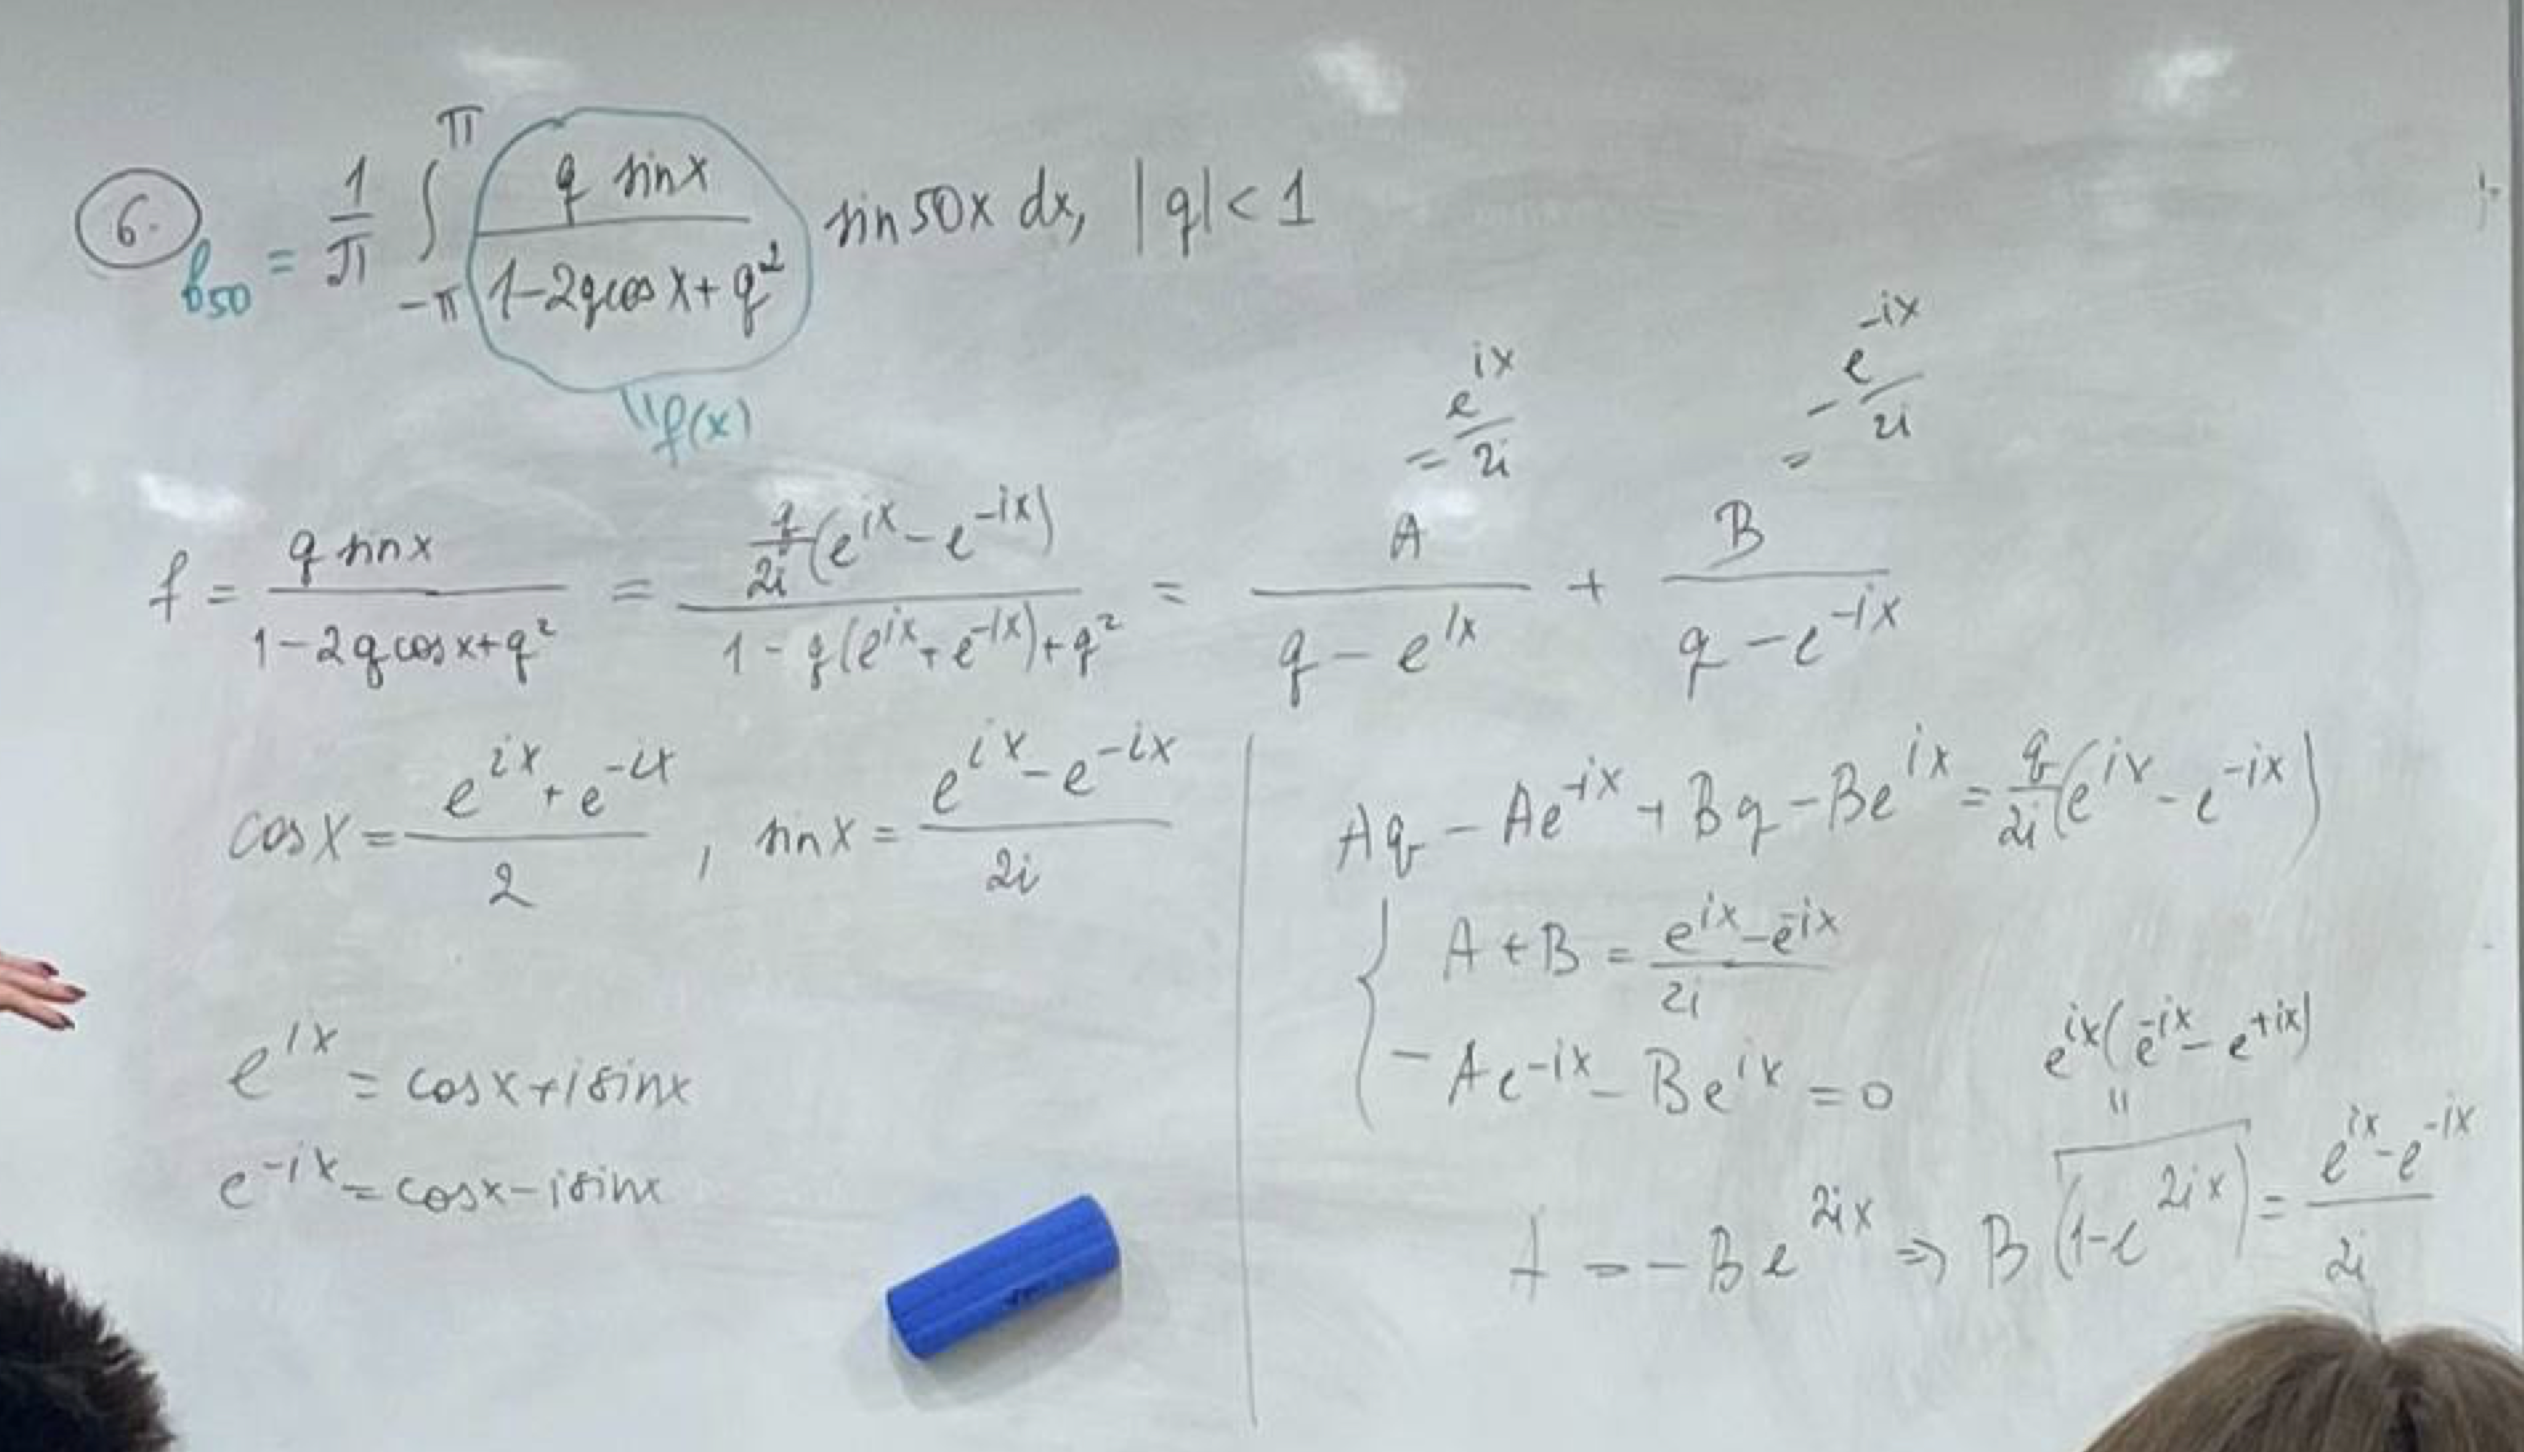
\includegraphics[scale=0.3]{3.png}
\end{center}
\begin{center}
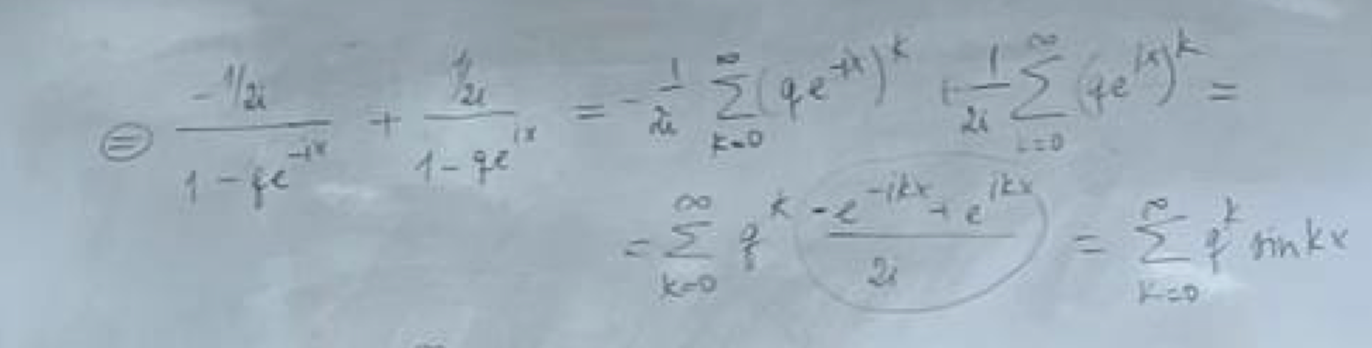
\includegraphics[scale=0.5]{4.png}
\end{center}
Очень хочется получить что-то аналогичное в числителе, добавим и вычтем сверху до знаменателя (чтобы вынести отдельно 1), чтобы там был косинус:
\[
\frac{1-q^2}{1-2q \cos x + q^2} = \frac{1-q^2 + 2q\cos x - 2q\cos x + (-1) - (-1)}{1-2q \cos x + q^2} =
\]
\[
= \frac{-(1 - 2q\cos x +q^2) - 2q\cos x + 1 - (-1)}{1-2q \cos x + q^2}  =
-1 + \frac{-2q \cos x + 2}{1 - 2q \cos x + q^2} =
\]
А теперь делаем как в 6м номере с семинара:
\[
=
-1 + \frac{-q (e^{ix}  + e^{-ix}) + 2}{1 - q (e^{ix}  + e^{-ix}) + q^2} = -1 + \left(
\frac{A}{q - e^{ix}} + \frac{B}{q - e^{-ix}}
\right) = (\times)
\]
Ищем коэффы:
\[
Aq - Ae^{-ix} + Bq - Be^{ix} = -q (e^{ix}  + e^{-ix}) + 2
\]
\[
\begin{cases}
A + B = -(e^{ix}  + e^{-ix}) \\
- Ae^{-ix} - Be^{ix}  = 2
\end{cases}
\]
\[
\begin{cases}
A = -e^{ix} \\
B = -e^{-ix}
\end{cases}
\]
Возвращаемся:
\[
(\times) = -1 + \frac{-e^{ix}}{q - e^{ix}} + \frac{-e^{-ix}}{q - e^{-ix}} = -1 + \frac{1}{1 - qe^{-ix}} + \frac{1}{1 - qe^{ix}} = -1 + \sum_{k = 0}^{\infty} \left( qe^{-ix} \right)^k + \sum_{k = 0}^{\infty} \left( qe^{ix} \right)^k   =
\]
\[
= -1 + 2\sum_{k = 0}^{\infty}  q^k \frac{e^{ikx} + e^{-ikx}}{2} = -1 + \sum_{k = 0}^{\infty} 2 q^k \cdot \cos (kx)
\]
Функцию разложили, теперь вычисляем:
\[
\frac{1}{\pi} \int\limits_{-\pi}^{\pi} \frac{1-q^2}{1-2q\cos x + q^2 } \cos (2022x)dx = a_{2022} =  2q^{2022}
\]
\begin{center}
\textbf{Ответ: } 

ряд фурье:
\[
-1 + 2 \sum_{k = 0}^{\infty} q^k \cdot \cos (kx)
\]
интеграл:
\[
2q^{2022}
\]
\end{center}
\end{document}
